%%----------------------------------------------------------------------------------------
\clearpage
\pagestyle{fancy}
%%----------------------------------------------------------------------------------------
%%       PREFAZIONE
%%----------------------------------------------------------------------------------------
\part{Strutture reticolari}
\setcounter{section}{0}
\section{La risoluzione grafica (Metodo dei nodi)}
%----------------------------------------------------------------------------------------
\noindent Nelle strutture reticolari l'elemento rigido è la \textsc{maglia triangolare}. Abbiamo già detto che una maglia triangolare oppure un complesso di maglie triangolari aventi in comune l'una con l'altra un lato, costituiscono \textsc{blocchi rigidi}. 
%----------------------------------------------------------------------------------------

\noindent Se le forze attive, come praticamente accade quasi sempre, sono \textsc{concentrate nei nodi}, è decisamente conveniente porsi nell'ottica seguente: le parti costituenti sono i \textsc{nodi cerniera} e le aste si considerano vincoli interni che collegano fra loro i \textsc{nodi}. Vale, ovviamente, la relazione 
%----------------------------------------------------------------------------------------
\begin{equation*}
m-n = l-i
\end{equation*}
%----------------------------------------------------------------------------------------
dove
%----------------------------------------------------------------------------------------
\begin{align*}
m &= \textup{Numero delle equazioni} = 2\forall\,\textup{\textsc{nodo}} \\
n &= \textup{Numero delle incognite} = 1\forall\,\textup{\textsc{asta}}+\textup{\textsc{reazioni vincolari esterne}}
\end{align*}
%----------------------------------------------------------------------------------------
Per determinare $l$ conviene cercare i centri assoluti e relativi; prima bisogna, però, individuare i \textsc{blocchi rigidi} all'interno della struttura ed ogni blocco rigido verrà assimilato ad un tronco. Trovato $l$ ed essendo $m$ ed $n$ noti \emph{a vista}, si può dunque classificare la struttura. Se essa è \textsc{staticamente determinata}, cioè se $i=0$, si possono ricavare le reazioni vincolari e gli sforzi nelle aste imponendo l'equilibrio nei \textsc{nodi} e l'equilibrio \textsc{esterno}. Vale la pena sottolineare che l'equilibrio di un \textsc{nodo}, che possiamo considerare come un \textsc{punto materiale}, si traduce nelle due equazioni di equilibrio alla traslazione; il suddetto equilibrio, come è noto, può anche esprimersi \textsc{graficamente} col fatto che le forze agenti sul \textsc{nodo} devono \textsc{chiudere il poligono} (delle forze, appunto). Ecco come conviene procedere: 
%----------------------------------------------------------------------------------------
\begin{enumerate}
%----------------------------------------------------------------------------------------
\item se la struttura è \textsc{isostatica per vincoli esterni}, si comincia ad imporre l'equilibrio esterno e si trovano così, agevolmente, le \textsc{reazioni di terra}, anche dette \textsc{reazioni esterne}; dopo di che si passa ad imporre, analiticamente o graficamente, l'\textsc{equilibrio} di quei nodi che risulteranno, via via, \textsc{staticamente determinati}, cioè quei nodi a cui corrispondono $2$ \textsc{incognite};
%----------------------------------------------------------------------------------------
\item se la struttura è \textsc{iperstatica per vincoli esterni} allora conviene procedere verificando le possibilità successive, come si è detto nei paragrafi precedenti e tenendo presente che nelle travature reticolari le \emph{vie} praticabili sono l'\textsc{equilibrio di un nodo} oppure l'\textsc{equilibrio di un blocco rigido}. 
%----------------------------------------------------------------------------------------
\end{enumerate}
%----------------------------------------------------------------------------------------
\section{Il metodo di Ritter}
%--------------------------------------------------------------------------------------------------------------------------------------------------------------
\renewcommand{\thefigure}{9~-~1}
\begin{figure}[ht]
\centering
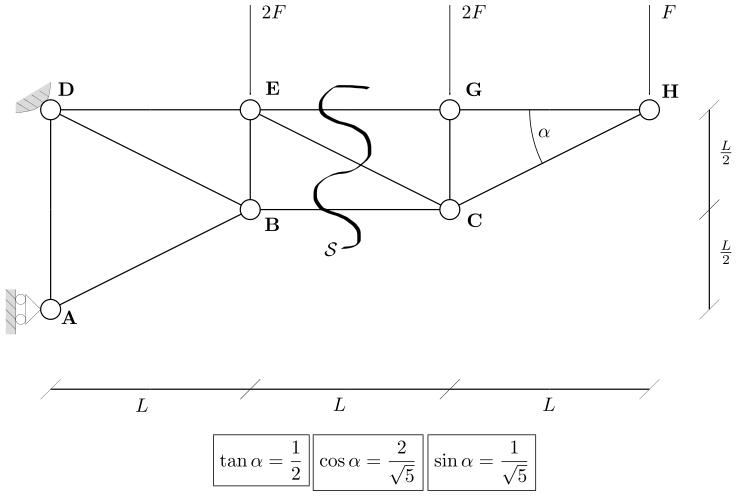
\includegraphics[width=\textwidth]{Immagini/Parte_9/Figura9_1/Figura9_1.pdf}
\caption{}
\label{figura9-1}
\end{figure}
%--------------------------------------------------------------------------------------------------------------------------------------------------------------
%----------------------------------------------------------------------------------------
Per capire meglio lo spirito del \textbf{Metodo di Ritter}, facciamo riferimento alla struttura reticolare rappresentata in figura~\ref{figura9-1}. Cominciamo a classificarla:
%----------------------------------------------------------------------------------------
\begin{align*}
m &= 2\forall\,\textup{\textsc{nodo}} = 2\times 7 = 14 \\
n &= 1\forall\,\textup{\textsc{asta}}+\textup{\textsc{Reazioni esterne}} = 3\,\,\textup{Esterne} + 11 = 14
\end{align*}
%----------------------------------------------------------------------------------------
e duque 
%----------------------------------------------------------------------------------------
\begin{equation*}
m-n = l-i = 0
\end{equation*}
%----------------------------------------------------------------------------------------
La struttura è costituita da cinque maglie triangolari aventi ciascuna un lato in comune con l'altra; si tratta pertanto di un unico \textsc{blocco rigido}. Osservando i vincoli esterni appare evidente che $l=0$ ed essendo $m-n=0$ allora si avrà che $i=0$. La strutura è dunque \textsc{isostatica}. Immaginiamo ora di sezionare la struttura come mostrato in figura: si sono ottenute, così, $2$ \textsc{parti} completamente disgiunte. Entrambe sono, ovviamente, in equilibrio. Si osservi che la sezione $S$ taglia $3$ aste che sono i vincoli interni colleganti l'una all'altra le $2$ parti suddette; se si considera ciascuna delle $2$ parti separate, e si segnano però su di esse le reazioni incognite delle aste che hanno subito il taglio, esse saranno sempre in equilibrio. Noi abbiamo disegnato la parte a destra della sezione del taglio $S$, perché su di essa le forze esterne sono tutte note e ciò rappresenta un notevole vantaggio. Abbiamo, ovviamente, disegnato anche gli sforzi incogniti nelle aste tagliate ipotizzandole tiranti.
%--------------------------------------------------------------------------------------------------------------------------------------------------------------
\renewcommand{\thefigure}{9~-~2}
\begin{figure}[ht]
\centering
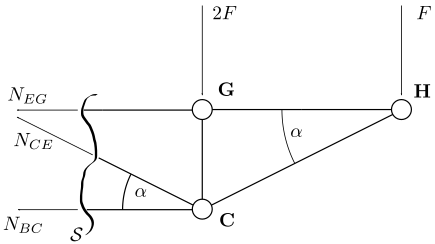
\includegraphics[width=0.6\textwidth]{Immagini/Parte_9/Figura9_2/Figura9_2.pdf}
\caption{}
\label{figura9-2}
\end{figure}
%--------------------------------------------------------------------------------------------------------------------------------------------------------------
%----------------------------------------------------------------------------------------
Poiché la parte in figura~\ref{figura9-2} è in equilibrio, le forze agenti su di essa dovranno verificare due equazioni di equilibrio alla traslazione, nonché l'equilibrio alla rotazione rispetto ad un polo qualunque. Si potrebbe scrivere una infinità di equazioni, cambiando la direzione della traslazione e cambiando polo, ben sapendo, tuttavia, che solo tre di esse sono \textsc{linearmente indipendenti}. E, allora, al fine di ricavare il più rapidamente possibile le tre incognite $N_{BC}$, $N_{CE}$ ed $N_{EG}$ noi vogliamo scrivere tre equazioni tali che in ciascuna di esse compaia $1$ \textsc{sola incognita}. Non ci vuole molto a scegliere le tre equazioni \emph{ad hoc}
%----------------------------------------------------------------------------------------
\begin{enumerate}
\item una equazione alla traslazione verso l'alto in cui figura solo $N_{CE}$;
\item una equazione alla rotazione con polo nel punto $\mathbf{C}$ (momenti considerati positivi in senso antiorario) in cui figura solo $N_{EG}$;
\item una equazione alla rotazione con polo nel punto $\mathbf{E}$ (momenti considerati positivi in senso antiorario) in cui figura solo $N_{BC}$.
\end{enumerate}
%----------------------------------------------------------------------------------------
E quindi:
%----------------------------------------------------------------------------------------
\begin{align*}
N_{CE}\sin{\alpha}-2F-F &= 0 \,\,\Rightarrow\,\, N_{CE} = \frac{3F}{\sin{\alpha}} = 3\sqrt{5}F \,\, (\textup{\textsc{Tirante}}) \quad [\uparrow] \\
N_{EG}\frac{L}{2}-FL &= 0 \,\,\Rightarrow\,\, N_{EG} = 2F \,\, (\textup{\textsc{Tirante}}) \quad [\mathbf{C}\circlearrowleft] \\
-N_{BC}\frac{L}{2}-2FL-2FL &= 0 \,\,\Rightarrow\,\, N_{BC} = -8F \,\, (\textup{\textsc{Puntone}}) \quad [\mathbf{E}\circlearrowleft] 
\end{align*}
%----------------------------------------------------------------------------------------
Alla luce dell'esempio appena svolto, dovrebbe ora risultare agevole comprendere il \textsc{metodo di Ritter}. 
%----------------------------------------------------------------------------------------

\noindent Dobbiamo premettere la seguente, fondamentale, definizione: 
%----------------------------------------------------------------------------------------
\begin{definizione}[\emph{di Sezione di Ritter}]
Si dice \textsc{sezione di Ritter relativa all'asta} $i$ ogni sezione che abbia i seguenti requisiti:
%----------------------------------------------------------------------------------------
\begin{enumerate}
\item divide la struttura in due parti disgiunte;
\item taglia l'asta $i$ ed almeno altre due aste;
\item tutte le aste tagliate tranne la $i$ devono concorrere in un punto o essere parallele.
\end{enumerate}
%----------------------------------------------------------------------------------------
\end{definizione}
%----------------------------------------------------------------------------------------
\noindent Ciò premesso, sarà possibile calcolare lo sforzo nell'asta $i$ con una sola, unica equazione se 
%----------------------------------------------------------------------------------------
\begin{itemize}
\item esiste \textsc{una sezione di Ritter relativa all'asta} $i$;
\item sono note le forze esterne su almeno una delle due parti nelle quali la struttura è stata sezionata. 
\end{itemize}
%----------------------------------------------------------------------------------------
Il procedimento è ovvio: si considera una delle due parti in cui la struttura è stata sezionata, scelta \emph{a piacere} purché siano note su di essa tutte le forze esterne e se ne scrive l'equazione di equilibrio \emph{ad hoc}.
%--------------------------------------------------------------------------------------------------------------------------------------------------------------
\clearpage
\section{Esercizi}
\paragraph{Esercizio 9.1}
%--------------------------------------------------------------------------------------------------------------------------------------------------------------
Determinare, con il \textsc{metodo dei nodi}, le reazioni vincolari e gli sforzi nelle aste della struttura esaminata nelle pagine precedenti e riportate in figura~\ref{Esercizio9-1-1}. 
%--------------------------------------------------------------------------------------------------------------------------------------------------------------
%--------------------------------------------------------------------------------------------------------------------------------------------------------------
\renewcommand{\thefigure}{9.1~-~1}
\begin{figure}[h!]
\centering
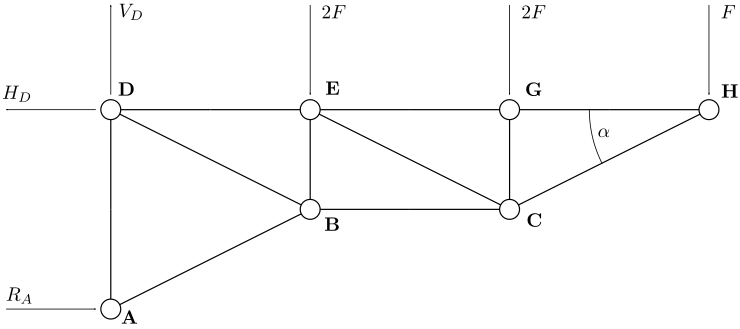
\includegraphics[width=\textwidth]{Immagini/Parte_9/Esercizio9_1/Esercizio9_1_1.pdf}
\caption{}
\label{Esercizio9-1-1}
\end{figure}

\noindent Cominciamo dall'equilibrio esterno, visto che la struttura è isostatica per vincoli esterni:
%----------------------------------------------------------------------------------------
\begin{align*}
R_A - H_D &= 0 \quad [\rightarrow] \\
V_D - 5F &= 0 \quad [\uparrow] \\ 
R_{A}\cdot L-2F\cdot L-2F\cdot2L - F\cdot3L &= \quad [\mathbf{D}\circlearrowleft] 
\end{align*}
%----------------------------------------------------------------------------------------
\noindent Si trova agevolmente le seguenti:
%----------------------------------------------------------------------------------------
\begin{align*}
R_A &= 9F \quad [\rightarrow] \\
H_D &= 9F \quad [\leftarrow] \\ 
V_D &= 5F \quad [\uparrow] 
\end{align*}
%----------------------------------------------------------------------------------------
%--------------------------------------------------------------------------------------------------------------------------------------------------------------
\renewcommand{\thefigure}{9.1~-~2}
\begin{figure}[ht]
\centering
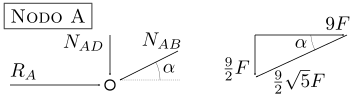
\includegraphics[width=0.45\textwidth]{Immagini/Parte_9/Esercizio9_1/Esercizio9_1_2.pdf}
\caption{}
\label{Esercizio9-1-2}
\end{figure}
%--------------------------------------------------------------------------------------------------------------------------------------------------------------
\noindent Ed ora andiamo ad imporre l'equilibrio nodo per nodo; possiamo partire dal nodo $\mathbf{A}$ o dal nodo $\mathbf{H}$, che sono entrambi staticamente determinati; possiamo procedere analiticamente o graficamente. Procediamo graficamente. 

\noindent Dalla figura~\ref{Esercizio9-1-2} notiamo che le forze $N_{AB}$ ed $N_{AD}$ segnate nel poligono delle forze rappresentano le azioni delle aste sul nodo $\mathbf{A}$. Si ricava agevolmente che
%----------------------------------------------------------------------------------------
\begin{align*}
N_{AD} &= \frac{9}{2}F \quad (\textup{\textsc{Tirante}}) \\
N_{AB} &= \frac{9}{2}\sqrt{5}F \quad (\textup{\textsc{Puntone}}) 
\end{align*}
%----------------------------------------------------------------------------------------
Imponiamo anche l'equilibrio del nodo $\mathbf{H}$, rappresentato in figura~\ref{Esercizio9-1-3}. Si ottiene agevolmente le seguenti
%----------------------------------------------------------------------------------------
\begin{align*}
N_{GH} &= 2F \quad (\textup{\textsc{Tirante}}) \\
N_{CH} &= \sqrt{5}F \quad (\textup{\textsc{Puntone}}) 
\end{align*}
%----------------------------------------------------------------------------------------
%--------------------------------------------------------------------------------------------------------------------------------------------------------------
\renewcommand{\thefigure}{9.1~-~3}
\begin{figure}[ht]
\centering
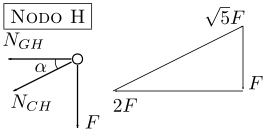
\includegraphics[width=0.45\textwidth]{Immagini/Parte_9/Esercizio9_1/Esercizio9_1_3.pdf}
\caption{}
\label{Esercizio9-1-3}
\end{figure}
%--------------------------------------------------------------------------------------------------------------------------------------------------------------
Via via che si ricavano gli sforzi nelle aste conviene segnarle sulla struttura: così apparirà evidente, ogni volta che è stato imposto l'equilibrio di un nodo, qual è il nodo che potremo successivamente considerare. A questo punto, la situazione è rappresentata in figura~\ref{Esercizio9-1-4}.
%--------------------------------------------------------------------------------------------------------------------------------------------------------------
\renewcommand{\thefigure}{9.1~-~4}
\begin{figure}[ht]
\centering
\includegraphics[width=\textwidth]{Immagini/Parte_9/Esercizio9_1/Esercizio9_1_4.pdf}
\caption{}
\label{Esercizio9-1-4}
\end{figure}
%--------------------------------------------------------------------------------------------------------------------------------------------------------------
Possiamo, dunque, gestire l'equilibrio del nodo $\mathbf{G}$ o $\mathbf{D}$; chiaramente è meglio $\mathbf{G}$. La figura~\ref{Esercizio9-1-5} mostra la situazione del nodo $\mathbf{G}$; si ricava facilmente quanto segue
%--------------------------------------------------------------------------------------------------------------------------------------------------------------
\renewcommand{\thefigure}{9.1~-~5}
\begin{figure}[ht]
\centering
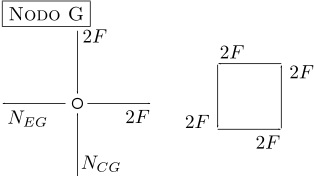
\includegraphics[width=0.45\textwidth]{Immagini/Parte_9/Esercizio9_1/Esercizio9_1_5.pdf}
\caption{}
\label{Esercizio9-1-5}
\end{figure}
%--------------------------------------------------------------------------------------------------------------------------------------------------------------
%----------------------------------------------------------------------------------------
\begin{align*}
N_{CG} &= 2F \quad (\textup{\textsc{Puntone}}) \\
N_{EG} &= 2F \quad (\textup{\textsc{Tirante}}) 
\end{align*}
%----------------------------------------------------------------------------------------
Ora andiamo ad imporre l'equilibrio del nodo $\mathbf{C}$; conviene preventivamente scomporre le forze note e sommare le componenti, come mostrato in figura~\ref{Esercizio9-1-6}, ottenendo infine:
%--------------------------------------------------------------------------------------------------------------------------------------------------------------
\renewcommand{\thefigure}{9.1~-~6}
\begin{figure}[ht]
\centering
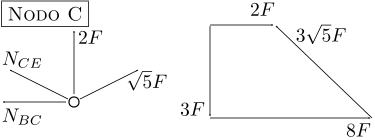
\includegraphics[width=0.45\textwidth]{Immagini/Parte_9/Esercizio9_1/Esercizio9_1_6.pdf}
\caption{}
\label{Esercizio9-1-6}
\end{figure}
%--------------------------------------------------------------------------------------------------------------------------------------------------------------
%----------------------------------------------------------------------------------------
\begin{align*}
N_{CE} &= 3\sqrt{5}F \quad (\textup{\textsc{Tirante}}) \\
N_{EG} &= 8F \quad (\textup{\textsc{Puntone}}) 
\end{align*}
%----------------------------------------------------------------------------------------
%--------------------------------------------------------------------------------------------------------------------------------------------------------------
\renewcommand{\thefigure}{9.1~-~7}
\begin{figure}[ht]
\centering
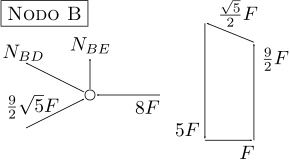
\includegraphics[width=0.45\textwidth]{Immagini/Parte_9/Esercizio9_1/Esercizio9_1_7.pdf}
\caption{}
\label{Esercizio9-1-7}
\end{figure}
%--------------------------------------------------------------------------------------------------------------------------------------------------------------
Andiamo ad imporre l'equilibrio del nodo $\mathbf{B}$; come mostrato in figura~\ref{Esercizio9-1-7}, anche qui si sono scomposte preventivamente le forze note e sommato le componenti, ottenendo
%----------------------------------------------------------------------------------------
\begin{align*}
N_{BD} &= \frac{\sqrt{5}}{2}F \quad (\textup{\textsc{Tirante}}) \\
N_{EG} &= 5F \quad (\textup{\textsc{Puntone}}) 
\end{align*}
%----------------------------------------------------------------------------------------
%--------------------------------------------------------------------------------------------------------------------------------------------------------------
\renewcommand{\thefigure}{9.1~-~8}
\begin{figure}[h!]
\centering
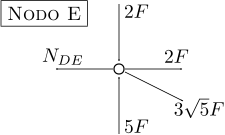
\includegraphics[width=0.45\textwidth]{Immagini/Parte_9/Esercizio9_1/Esercizio9_1_8.pdf}
\caption{}
\label{Esercizio9-1-8}
\end{figure}
%--------------------------------------------------------------------------------------------------------------------------------------------------------------
Infine, andiamo ad imporre il nodo $\mathbf{E}$, come mostrato in figura~\ref{Esercizio9-1-8}; sono ormai note tutte le forze tranne $N_{DE}$, per cui si ha una somma di forze tutte note. La somma di tutte le componenti verticali è nulla mentre quella delle componenti orizzontali vale $8F$. Ciò è perfettamente compatibile con l'equilibrio del nodo $\mathbf{E}$; l'asta $\mathbf{D}\mathbf{E}$, dunque, reagirà con la seguente forza
%----------------------------------------------------------------------------------------
\begin{equation*}
N_{DE} = 8F \quad (\textup{\textsc{Tirante}}) 
\end{equation*}
%----------------------------------------------------------------------------------------
A questo punto sono noti tutti gli sforzi nelle aste e si può tracciare il quadro completo degli sforzi nelle aste, come mostrato in figura~\ref{Esercizio9-1-9}.
%--------------------------------------------------------------------------------------------------------------------------------------------------------------
\renewcommand{\thefigure}{9.1~-~9}
\begin{figure}[ht]
\centering
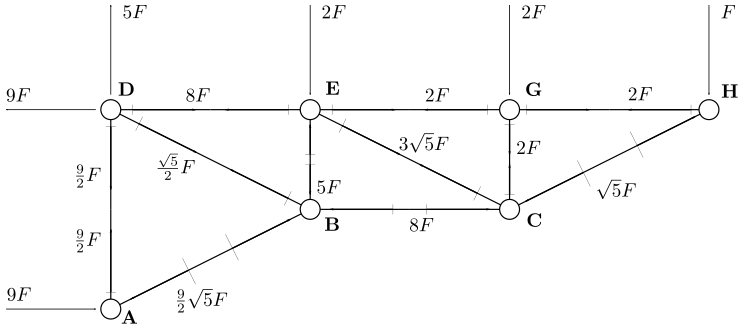
\includegraphics[width=\textwidth]{Immagini/Parte_9/Esercizio9_1/Esercizio9_1_9.pdf}
\caption{}
\label{Esercizio9-1-9}
\end{figure}
%--------------------------------------------------------------------------------------------------------------------------------------------------------------
Vale la pena sottolineare che non è stato mai imposto l'equilibrio del nodo $\mathbf{D}$; tale equilibrio si può adoperare come strumento di verifica:
%----------------------------------------------------------------------------------------
\begin{align*}
-9F + 8F + \frac{\sqrt{5}}{2}F\cos{\alpha} &= 0 \quad [\rightarrow] \quad \textup{\textsc{Ok!}} \\
-\frac{9}{2}F + 5F -\frac{\sqrt{5}}{2}F\sin{\alpha} &= 0 \quad [\uparrow]  \quad \textup{\textsc{Ok!}}
\end{align*}
%----------------------------------------------------------------------------------------
Osserviamo, infine, come gli sforzi ora trovati per le aste $\mathbf{B}\mathbf{C}$, $\mathbf{C}\mathbf{E}$ ed $\mathbf{E}\mathbf{G}$ coincidano in valore e verso con quelli trovati con il \textsc{metodo di Ritter} in precedenza.
%----------------------------------------------------------------------------------------
%----------------------------------------------------------------------------------------
%----------------------------------------------------------------------------------------
%----------------------------------------------------------------------------------------
%----------------------------------------------------------------------------------------
%----------------------------------------------------------------------------------------
%----------------------------------------------------------------------------------------
%----------------------------------------------------------------------------------------
%----------------------------------------------------------------------------------------
%----------------------------------------------------------------------------------------
%----------------------------------------------------------------------------------------
%----------------------------------------------------------------------------------------
%----------------------------------------------------------------------------------------
%----------------------------------------------------------------------------------------
%----------------------------------------------------------------------------------------
%----------------------------------------------------------------------------------------
%----------------------------------------------------------------------------------------
%----------------------------------------------------------------------------------------
%----------------------------------------------------------------------------------------
%----------------------------------------------------------------------------------------
%----------------------------------------------------------------------------------------
%----------------------------------------------------------------------------------------
%----------------------------------------------------------------------------------------
%----------------------------------------------------------------------------------------
%----------------------------------------------------------------------------------------
%----------------------------------------------------------------------------------------
%----------------------------------------------------------------------------------------
%----------------------------------------------------------------------------------------
%----------------------------------------------------------------------------------------
%----------------------------------------------------------------------------------------
%----------------------------------------------------------------------------------------
